%%=============================================================================
%% Methodologie
%%=============================================================================

\chapter{Methodologie}
\label{ch:methodologie}

%% TODO: Hoe ben je te werk gegaan? Verdeel je onderzoek in grote fasen, en
%% licht in elke fase toe welke stappen je gevolgd hebt. Verantwoord waarom je
%% op deze manier te werk gegaan bent. Je moet kunnen aantonen dat je de best
%% mogelijke manier toegepast hebt om een antwoord te vinden op de
%% onderzoeksvraag.

Om een antwoord te vinden op de gestelde onderzoeksvragen dient er een experiment uitgevoerd te worden. Hoe dit experiment zal verlopen wordt hieronder nader verklaard.

\section{Plan van aanpak}

Het experiment zal grotendeels uitgevoerd worden op willekeurige testpersonen. Bij deze testpersonen zal er a.d.h.v. een wasknijper een pijnprikkel opgewekt worden. Deze pijnprikkel zal gedurende enkele oefensessies verdragen moeten worden.

Bij een eerste oefensessie zal de persoon 10 maal een beweging moeten uitvoeren met de wasknijper op de vinger. 
Tijdens de tweede oefensessie zal de persoon de VR bril en een hoofdtelefoon opgezet krijgen. Hier zal hij terechtkomen in 'ApplePicker', het gerealiseerde prototype voor dit onderzoek. In deze game zal de persoon opnieuw 10 maal een beweging moeten uitvoeren, met de wasknijper op de vinger.

Na elke oefensessie dient de persoon een vragenlijst in te vullen 
over zaken zoals: hoe de pijnervaring was tijdens de oefeningen, of de persoon zich altijd even gemotiveerd voelt om revalidatie oefeningen uit te voeren, ...

Ook zal er een experiment uitgevoerd worden op enkele testpersonen die momenteel lijden aan een letsel aan de bovenste ledematen. Opnieuw zullen er enkele oefensessies plaatsvinden, maar nu onder begeleiding van de kinesist.

Gedurende de eerste oefensessie zal de kinesist de testpersoon bijstaan bij het uitvoeren van de oefeningen zonder enige hulp van VR.
Bij de tweede oefensessie zal de persoon dan opnieuw de VR bril en de hoofdtelefoon opgezet krijgen. Deze keer zal de kinesist de bewegingen van de patiënt op het computerscherm kunnen volgen om mogelijke instructies te kunnen geven. Wanneer de kinesist dit wenst zijn er ook polsgewichten om de oefeningen wat uitdagender te maken voor de patiënt.

Ook hier zal de persoon nadien nog een vragenlijst moeten invullen.

\chapter{Experiment}

\section{Materiaal}
Om het experiment uit te voeren waren enkele zaken onmisbaar:

- VR headset en controller: Hier werd de Oculus Go gebruikt

- Computer: Hierop werden de vragenlijsten ingevuld na de oefensessies. Ook kon de kinesist/begeleider hierop meevolgen wat de patiënt in het spel aan het doen was.

- Polsgewichten (eventueel): Deze konden bij de patiënt omgedaan worden om de intensiteit van de oefeningen te vergroten.

\newpage
\subsection{Testpersonen}
Als testpersonen werden er 25 willekeurige personen gekozen tussen de 19 en 85 jaar. Op \cite{figuur 6.1} kan u bijhorende boxplot terugvinden van de verdeling van de leeftijden per geslacht. De testpersoon werd op voorhand niet ingelicht over de opzet van het onderzoek zodat ze onbevooroordeeld de vragen konden invullen.

\begin{figure}[h]
    \centering
    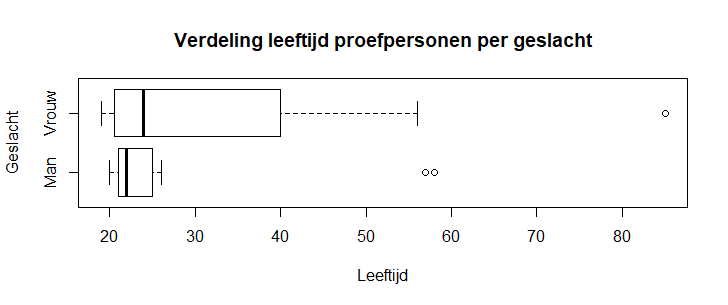
\includegraphics[scale=0.7]{Boxplot_Leeftijd.png}
    \caption{Boxplot van leeftijden van proefpersonen}
\end{figure}

Tijdens het experiment werd de proefpersoon een wasknijper opgedaan om een pijnprikkel te simuleren. Hierna diende de oefening uitgevoerd te worden (\cite{figuur 6.2}).

\begin{figure}[h]
    \centering
    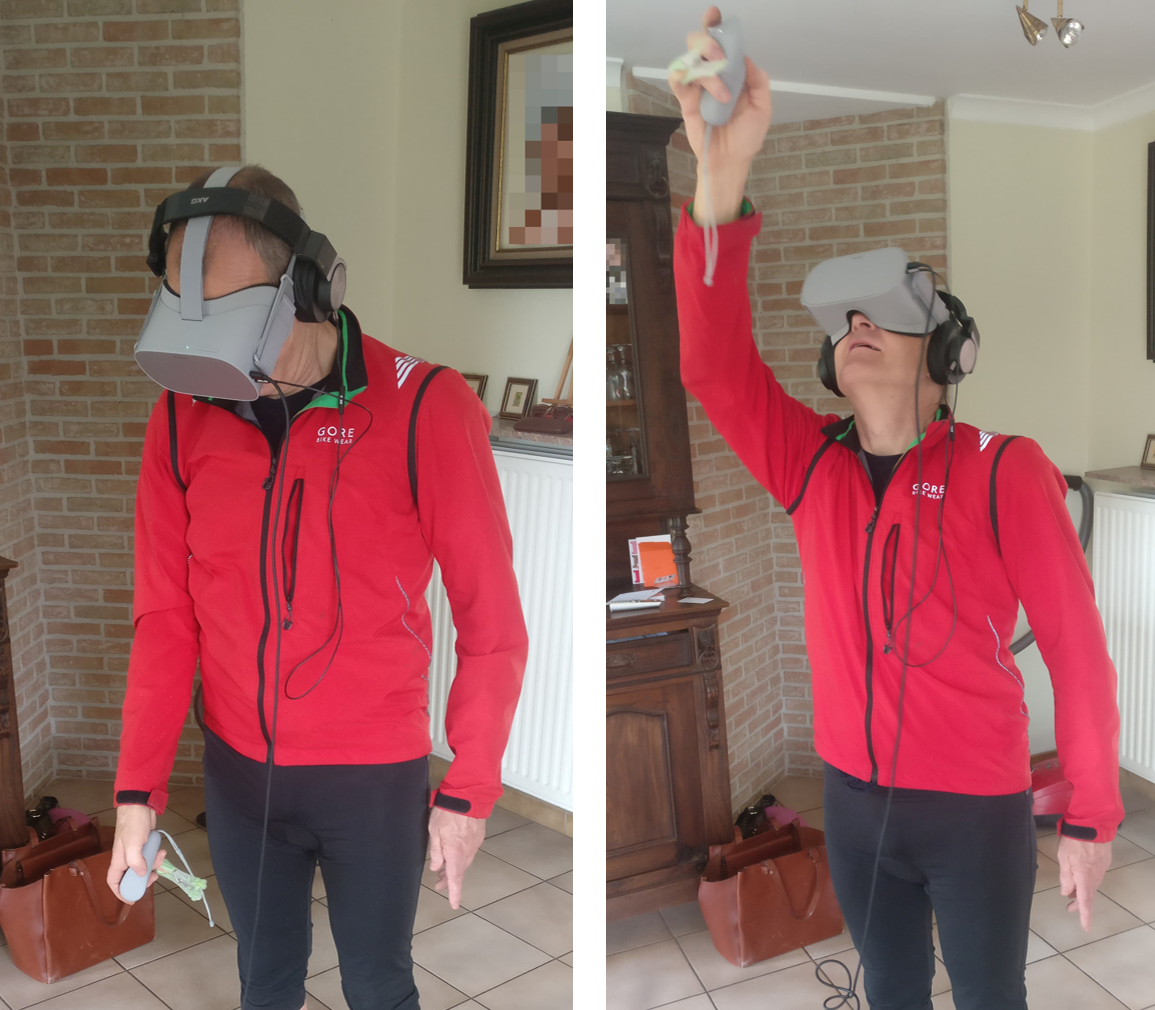
\includegraphics[scale=0.8]{luc.png}
    \caption{Proefpersoon test de applicatie met wasknijper op de vinger en voert de beweging uit}
\end{figure}

\newpage

\section{Resultaten}

\subsection{Verschil pijnervaring}

TODO: boxplot bespreken en gemiddelde afname berekenen.

\begin{figure}[h]
    \centering
    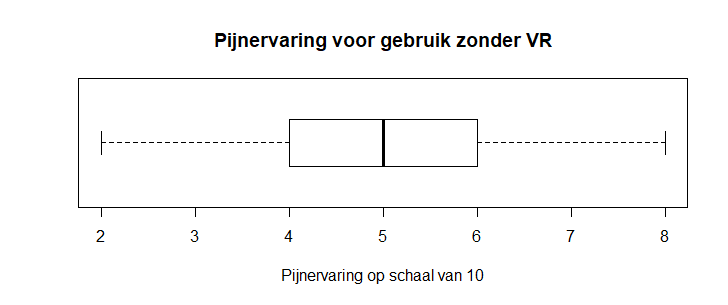
\includegraphics[scale=0.7]{boxplot_PijnZonder.png}
    \caption{Boxplot van pijnervaring testgebruikers na oefensesie zonder VR}
\end{figure}

\begin{figure}[h]
    \centering
    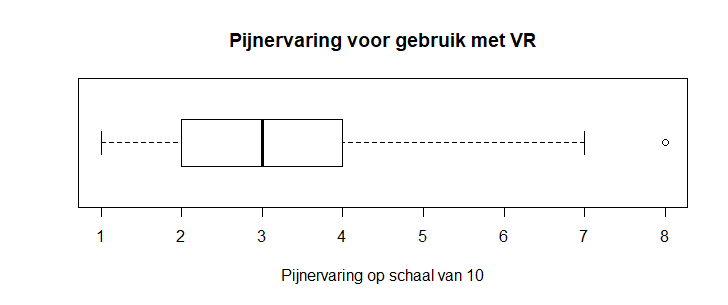
\includegraphics[scale=0.7]{boxplot_PijnMet.png}
    \caption{Boxplot van pijnervaring testgebruikers na oefensesie met VR}
\end{figure}



